\chapter{Conclusion}
The complete workflow consists of hardware and scheduler mentioned in the project are given in the following figure:-


\begin{figure}[H]
    \centering
    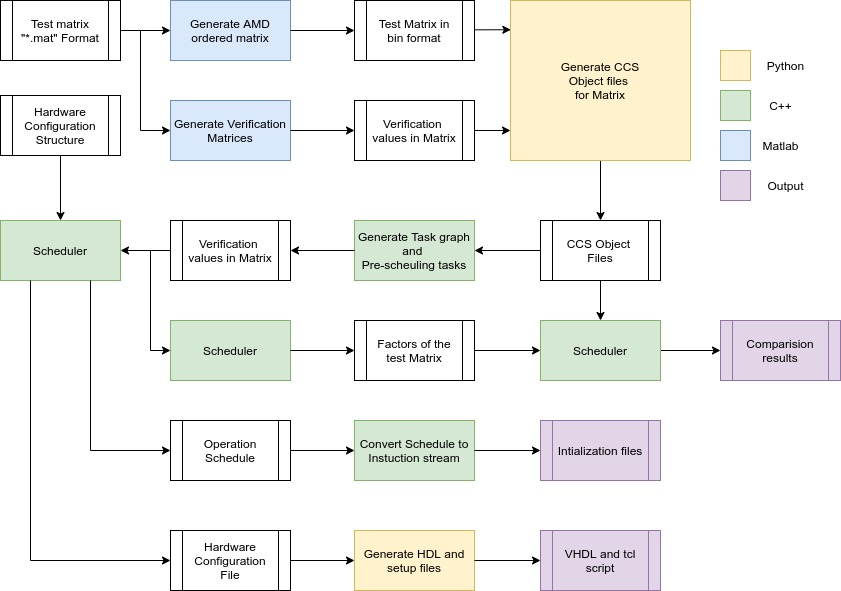
\includegraphics[width = \textwidth]{./Software/Workflow.jpg}
    \caption{Workflow of Software}
\end{figure}


The hardware is generated to an AXI wrapper IP such that it can be connectable with the Microblaze (soft-core processor)  or  ZynQ (hard-core processor) is generated. The following is the report of Dual Port IP hardware.\\



\begin{figure}[H]
    \centering
    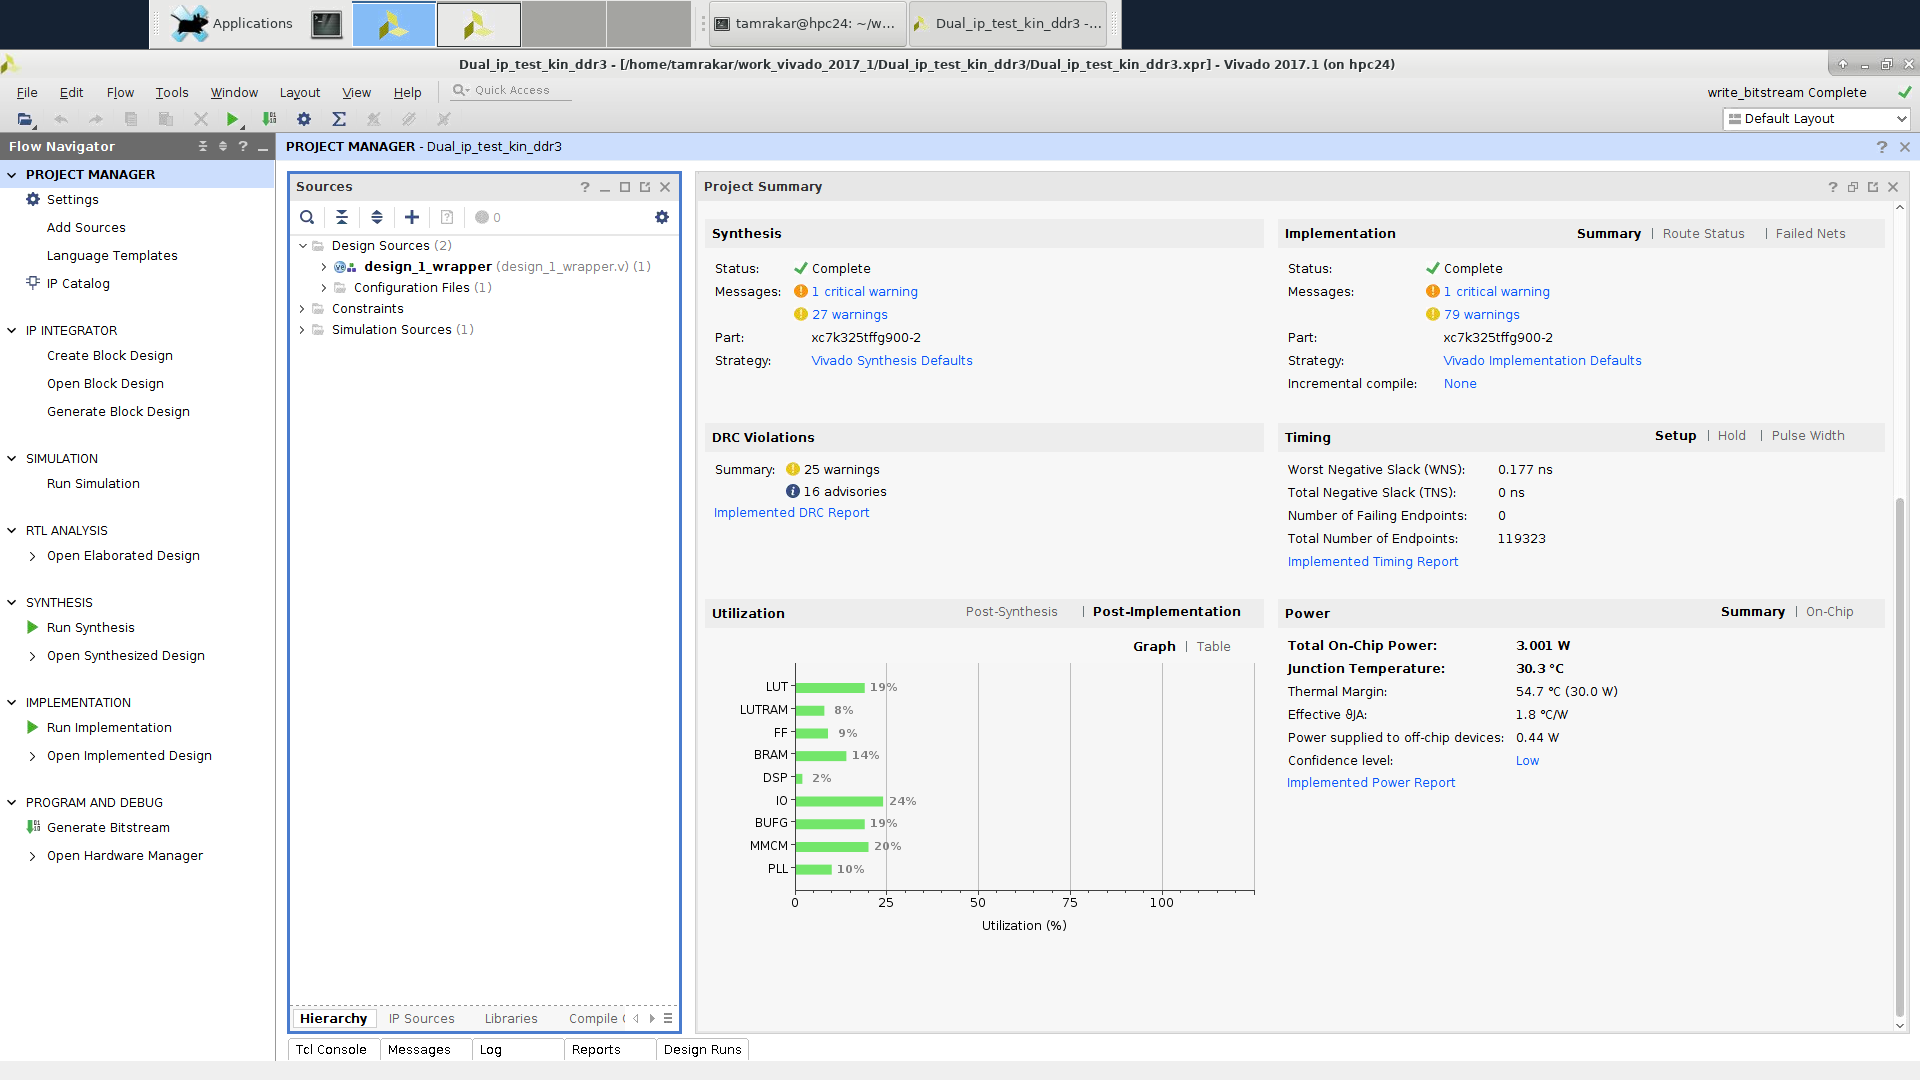
\includegraphics[width = \textwidth]{./Software/Report.png}
    \caption{IP generation report}
\end{figure}


The AXI wrapper hardware is connected to MicroBlaze and the necessary components to properly function on Kintex KC-705 Xilinx Board. A cache is attached to increase the efficiency of the executions. Following is the block-level design of the interconnections of hardware for Testing.\\



\begin{figure}[H]
    \centering
    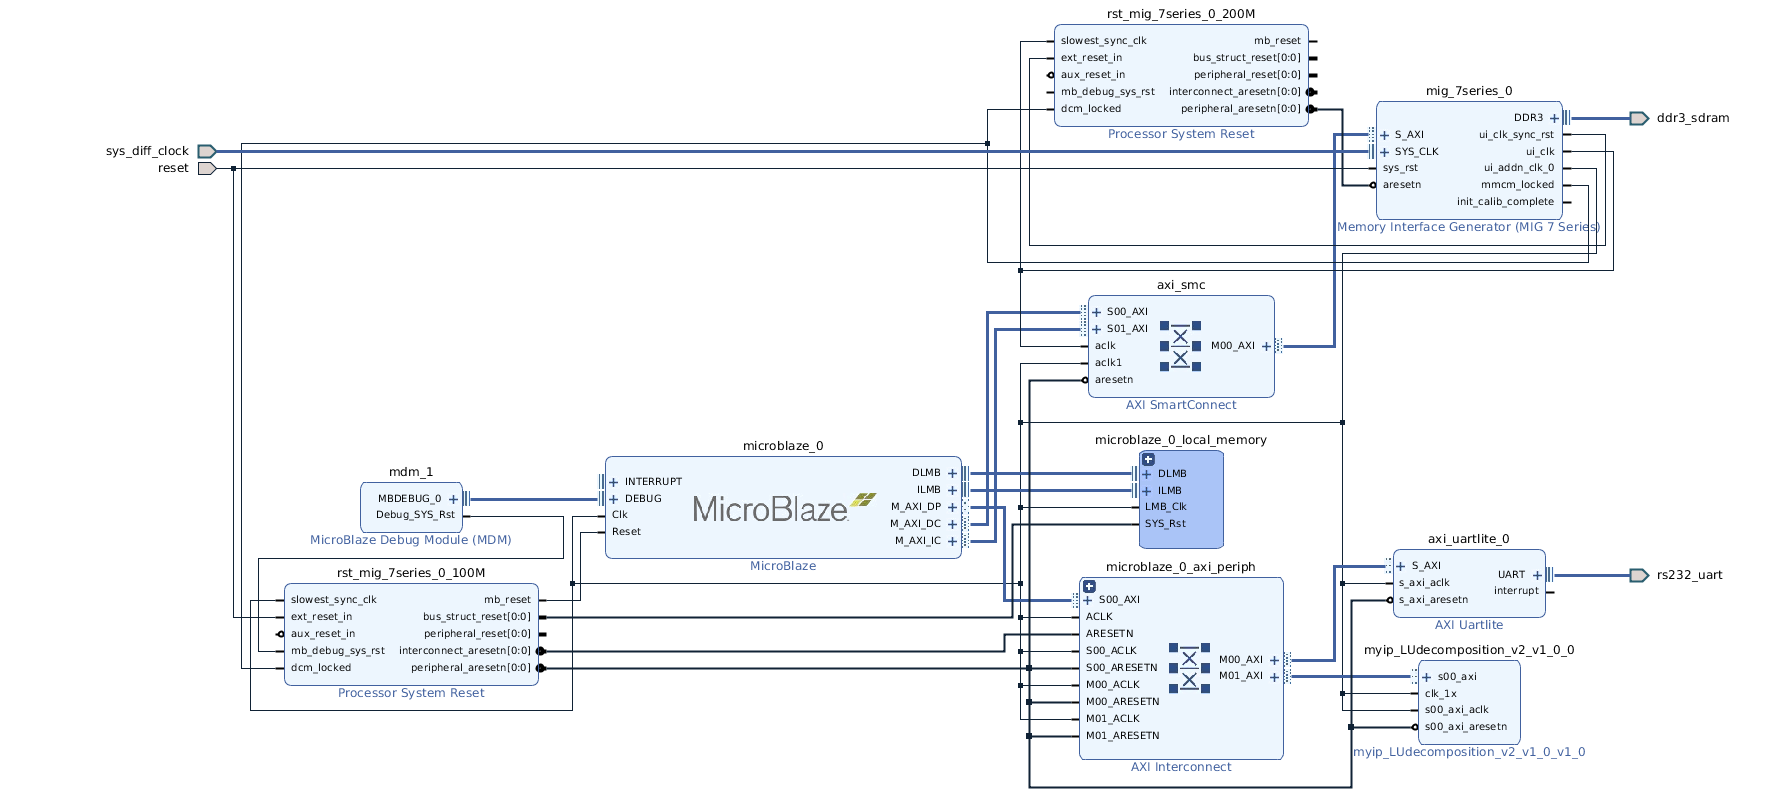
\includegraphics[width = \textwidth]{./Software/Schematic_.png}
    \caption{MicroBlaze interconnect}
\end{figure}

\pagebreak
Microblaze code generated by the schedule for uploading instructions and data stream is used for interfacing IP and MicroBlaze. This was implemented and tested successfully on the Kintex KC-705 board, and the output is taken from UART and verified with golden reference generated by MATLAB script.
\\
\\
Currently following are the scope for further improvements and implementation in the projects:-
\begin{itemize}
	\item Dynamic Scheduler
	\item ILP Based Scheduler 
	\item Scheduler for QR Decomposition
	\item Uniform Channel Decomposition for MIMO communication
	\item Generating ASIC Design 
    \item Integration with generic processor
\end{itemize}
Phase \Romannum{2} of the Project will converge to some of the improvements and implementation mentioned above.